% F(alpha) = 6 cos^2 alpha - 4 sin^2 alpha + 2 beta cos(alpha - 45 deg) along the circle of the worked example
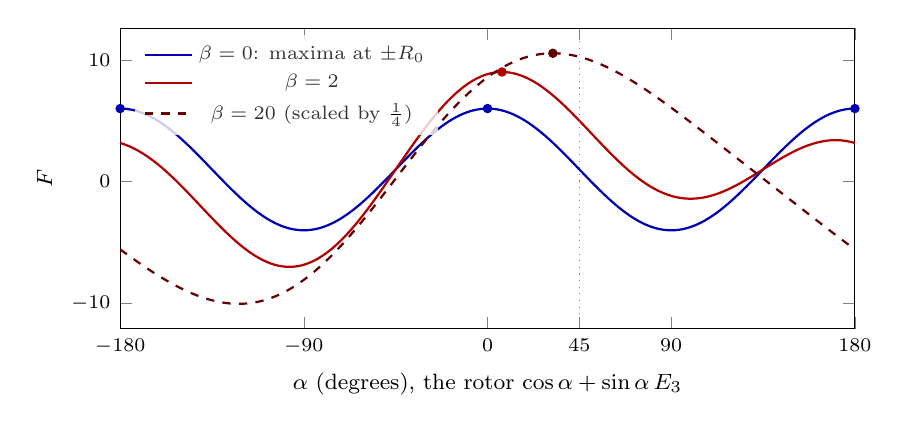
\begin{tikzpicture}
  \begin{axis}[width=0.9\textwidth, height=5.4cm, xmin=-180, xmax=180, xtick={-180,-90,0,45,90,180},
      xlabel={$\alpha$ (degrees), the rotor $\cos\alpha + \sin\alpha\, E_3$}, ylabel={$F$},
      legend style={at={(0.02,0.98)}, anchor=north west, font=\scriptsize, draw=none, fill=white, fill opacity=0.8},
      tick label style={font=\scriptsize}, label style={font=\footnotesize}, samples=361, domain=-180:180]
    \addplot[thick, blue!70!black] {6*cos(x)^2 - 4*sin(x)^2};
    \addplot[thick, red!70!black] {6*cos(x)^2 - 4*sin(x)^2 + 4*cos(x-45)};
    \addplot[thick, red!40!black, dashed] {(6*cos(x)^2 - 4*sin(x)^2 + 40*cos(x-45))/4};
    \addplot[only marks, mark=*, mark size=1.5pt, blue!70!black] coordinates {(0,6) (180,6) (-180,6)};
    \addplot[only marks, mark=*, mark size=1.5pt, red!70!black] coordinates {(7.1,9.0036)};
    \addplot[only marks, mark=*, mark size=1.5pt, red!40!black] coordinates {(32.0,10.5417)};
    \draw[gray, dotted] (axis cs:45,-12) -- (axis cs:45,12);
    \legend{{$\beta = 0$: maxima at $\pm R_0$}, {$\beta = 2$}, {$\beta = 20$ (scaled by $\frac14$)}}
  \end{axis}
\end{tikzpicture}
